\subsection{Concordia Pinner} \label{subsection:4-3-4-concordia-pinner-service}

\subsubsection{Περιγραφή - Στόχοι υπηρεσίας}

Η υπηρεσία καρφιτσώματος περιεχομένου (Concordia Pinner) αποτελεί μία εφαρμογή τερματικού (temrinal application/cmd application) η οποία στοχεύει στο καρφίτσωμα (pinning) του περιεχομένου που αποθηκεύεται στο IPFS μέσω της βάσης OrbitDB. Η υπηρεσία είναι γραμμένη στη γλώσσα προγραμματισμού Javascript. Η αρχιτεκτονική της υπηρεσίας φαίνεται το σχήμα \ref{figure:4-3-concordia-pinner-architecture}.

\begin{figure}[H]
    \centering
    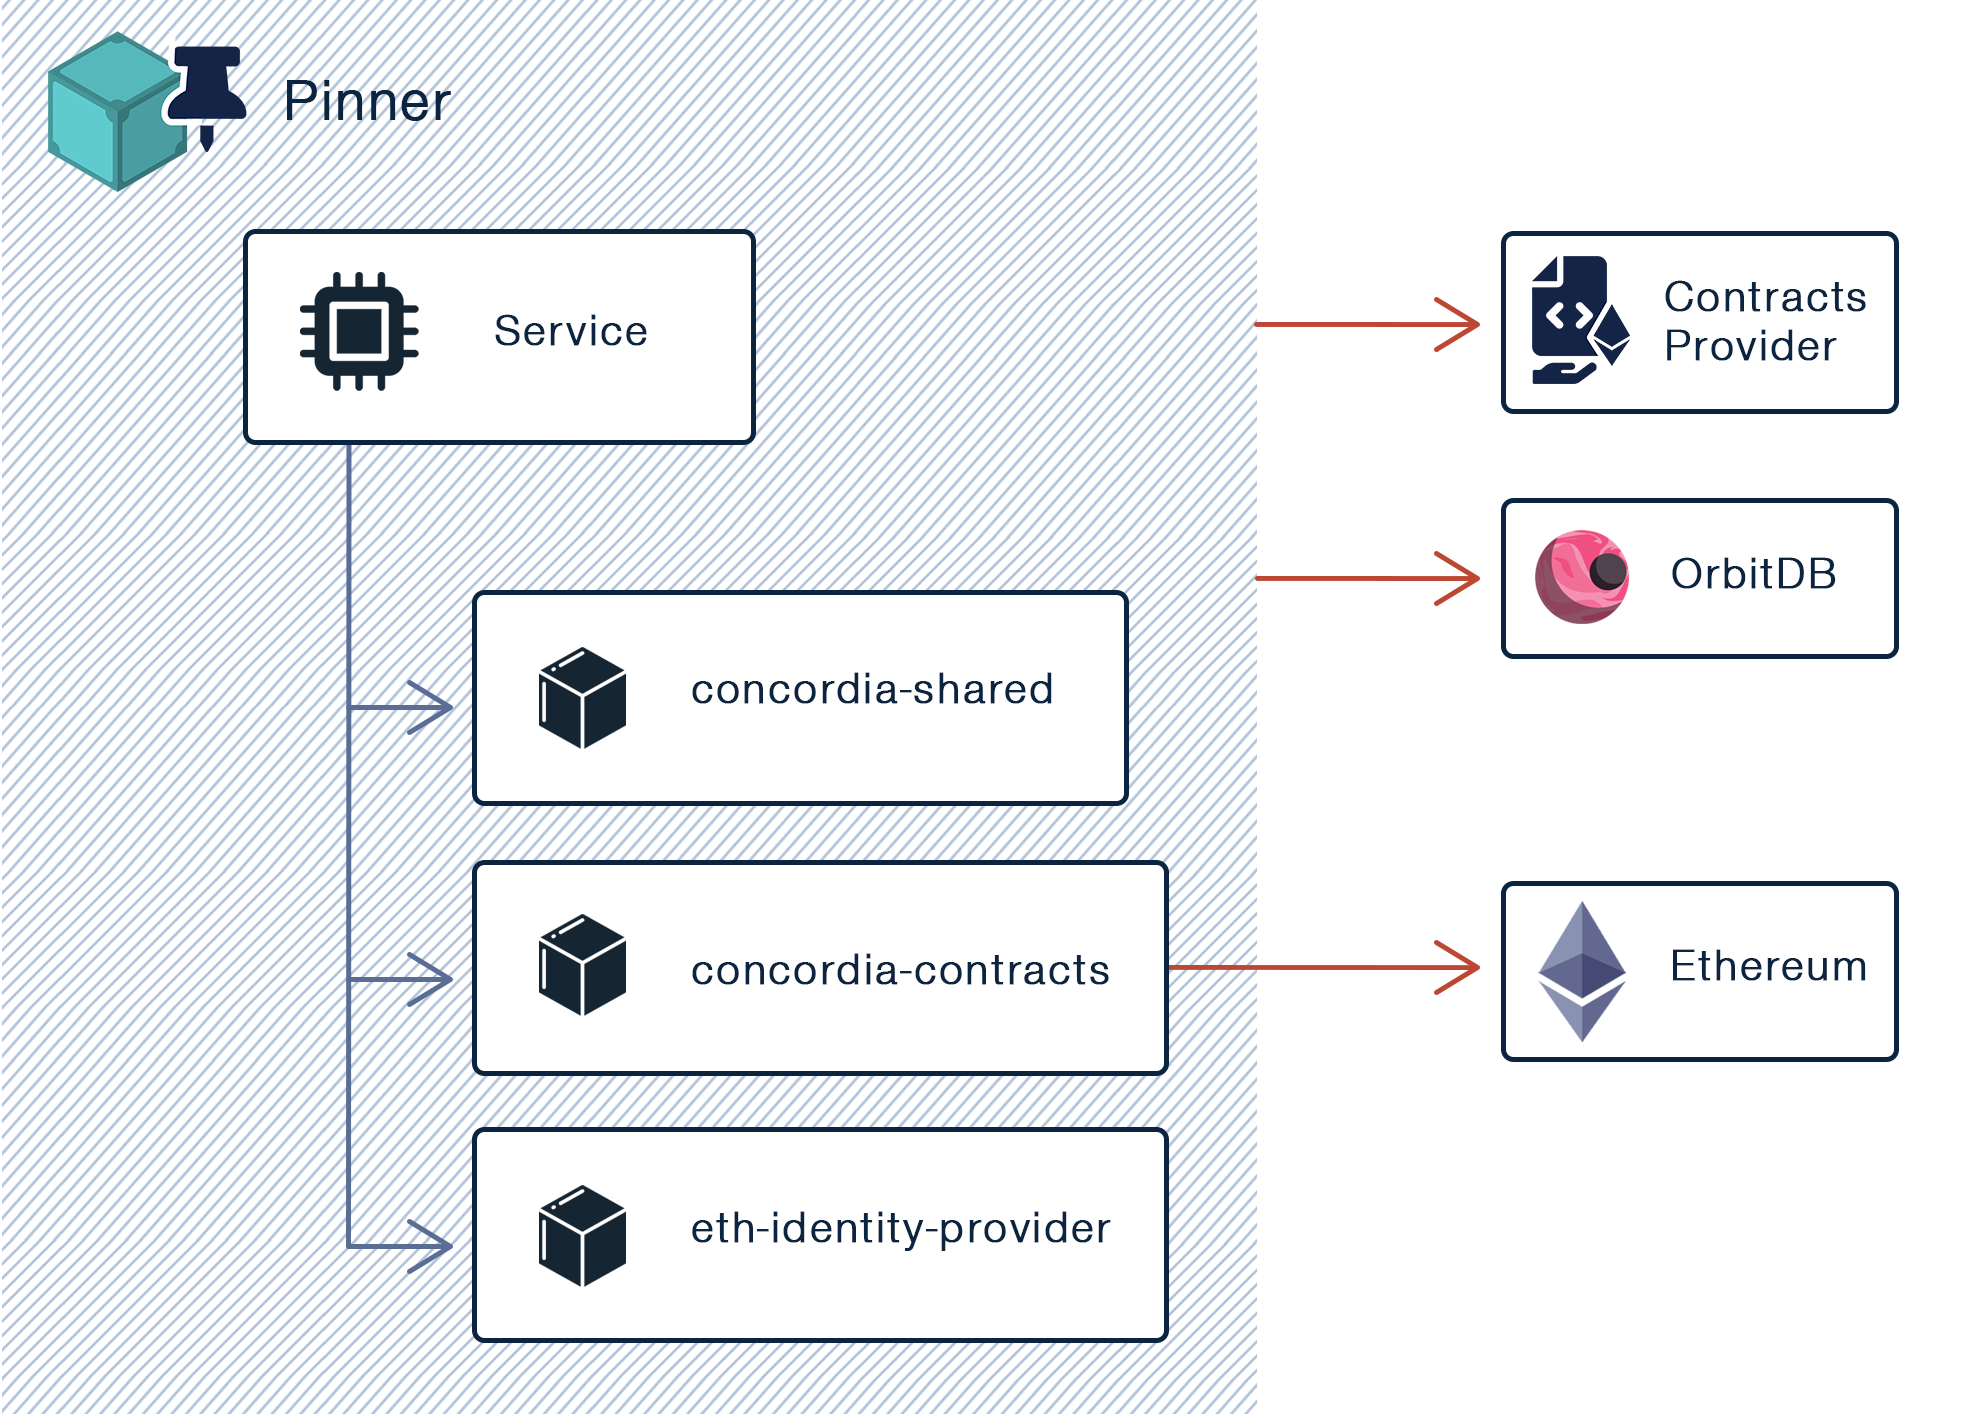
\includegraphics[width=.6\textwidth]{assets/figures/chapter-4/4.3.architecture-4.3.4.concordia-pinner-architecture.png}
    \caption{Αρχιτεκτονική υπηρεσίας Concordia Pinner}
    \label{figure:4-3-concordia-pinner-architecture}
\end{figure}

Η υπηρεσία αυτή υλοποιήθηκε για να εγγυηθεί η διαθεσιμότητα του περιεχομένου του συστήματος που αποθηκεύεται στο IPFS (τίτλοι θεμάτων, περιεχόμενο μηνυμάτων και άλλα). Λόγω του τρόπου λειτουργίας % todo: insert reference
του IPFS, το περιεχόμενο που αναρτούν οι χρήστες πρέπει να καρφιτσώνεται από άλλους χρήστες ή αυτόνομες εφαρμογές, όπως η υπηρεσία Concordia Pinner, ώστε να είναι διαθέσιμο. Αν το περιεχόμενο δεν καρφιτσωθεί, τότε θα είναι διαθέσιμο στους υπόλοιπους χρήστες μόνο από %todo: fix gender stuff
τον/τη δημιουργό, έτσι αν αυτός/αυτή δεν είναι ενεργός/ενεργή στο δίκτυο, το περιεχόμενο θα είναι αδύνατο να βρεθεί.

Η υπηρεσία συνδέεται στο blockchain από όπου παρακολουθεί την κατάσταση του συστήματος και ``ακούει'' για νέους χρήστες, θέματα και μηνύματα. Η υπηρεσία συνδέεται επίσης στο IPFS, έτσι όταν δημιουργηθεί νέο περιεχόμενο στο σύστημα το καρφιτσώνει αυτόματα. Με αυτό τον τρόπο, διατηρώντας την υπηρεσία πάντα διαθέσιμη, για παράδειγμα εκτελώντας τη σε περιβάλλον διακομιστή (server), διαβεβαιώνεται η διαθεσιμότητα του περιεχομένου.

\subsubsection{Διανομή}

Η υπηρεσία αυτή γίνεται διαθέσιμη για χρήση ως docker image μέσω του αποθετηρίου εικόνων dockerhub. Κατά την εκτέλεση της εικόνας οι χρήστες μπορούν μέσω μεταβλητών περιβάλλοντος να ορίσουν παραμέτρους της υπηρεσίας όπως τη διεύθυνση του εξυπηρετητή (host location), τη διεύθυνση του blockchain, τις διαδρομές αποθήκευσης των δεδομένων στο σύστημα και τις τοποθεσίες των υπηρεσιών Rendezvous Server και Contracts Provider.